\section{Equipamentos}
\label{sec:equipamentos}

	Como etapa inicial para o funcionamento da Realidade Aumentada, necessita-se de equipamentos que
	possuam a funcionalidade de captura de vídeo, como por exemplo~\textit{webcam's}. Esses
	proporcionam a captura do ambiente do usuário e envia os dados para um dispositivo responsável pelo
	processamento. Dentre os equipamentos utilizados inicialmente na Realidade Aumentada pode-se citar
	o~\textit{HMD (Head Mounted Display)}. Eles eram utilizados com o objetivo de captura das
	informações, através de suas câmeras acopladas, posteriormente processavam as informações
	necessárias e exibia o resultado do processamento ao usuário através de objetos virtuais
	visualizados em suas telas acopladas ao equipamento.
	
	Este equipamento é fixado na cabeça do usuário podendo ter o formato de um capacete ou de um
	óculos. Algumas utilidades desse equipamento pode ser encontrada em realizações de simulações
	computadorizadas e também para a visualização dos objetos virtuais ao qual o âmbito da Realidade
	Aumentada está inserida~\cite{ronaldAzuma}.
		
	Quando esse equipamento foi proposto, ele possuía algumas desvantagens por ser muito pesado e
	evasivo. Atualmente, projetos estão sendo desenvolvidos para tentar minimizar essas desvantagens. A
	figura~\ref{fig:hmd} mostra um equipamento~\textit{HMD} com características que favoreçam sua
	utilização. Por outro lado, a grande vantagem desse tipo de equipamento é a possibilidade de
	imersão do usuário em um ambiente onde ele consiga interagir entre o virtual e o real de uma forma
	mais natural.
	
	\begin{figure}[htb]
		\centering 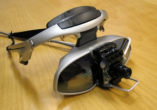
\includegraphics[scale=1.25]{figuras/cap2/hmd.jpg}
		\caption{\textit{Head Mounted Display ~\cite{nilsson}.}}
		\label{fig:hmd} 
	\end{figure}
	
	Atualmente, os \textit{smartphones} estão ganhando cada vez mais espaço dentro da Realidade
	Aumentada. Com a evolução do \textit{GPU (Graphics Processing Unit)} nestes, ocorreu a
	popularização de seu uso em aplicações voltadas para a Realidade Aumentada. A grande vantagem em
	sua utilização está na abrangência com que eles são distribuídos e principalmente na mobilidade
	conseguida através dos mesmos. Este equipamento comporta todos os recursos necessários para sua
	utilização na Realidade Aumentada:
	
	\begin{enumerate}
	  	\item A câmera do celular substitui a \textit{webcam} ou as câmeras acopladas ao HMD;
		\item O processamento gráfico é feito na~\textit{GPU};
		\item O resultado é apresentado no próprio visor do aparelho, suprindo a necessidade de um
		monitor ou telas para a visualização do objeto virtual.
	\end{enumerate}

	Um exemplo de utilização da Realidade Aumentada em \textit{smartphones} pode ser visto na
	figura~\ref{fig:arAndroid}. Nesta, a câmera do \textit{smartphone} captura a imagem do marcador,
	processa as informações necessárias e exibe um carro como objeto virtual correspondente para aquele
	marcador.
						
	\begin{figure}[htb]
		\centering 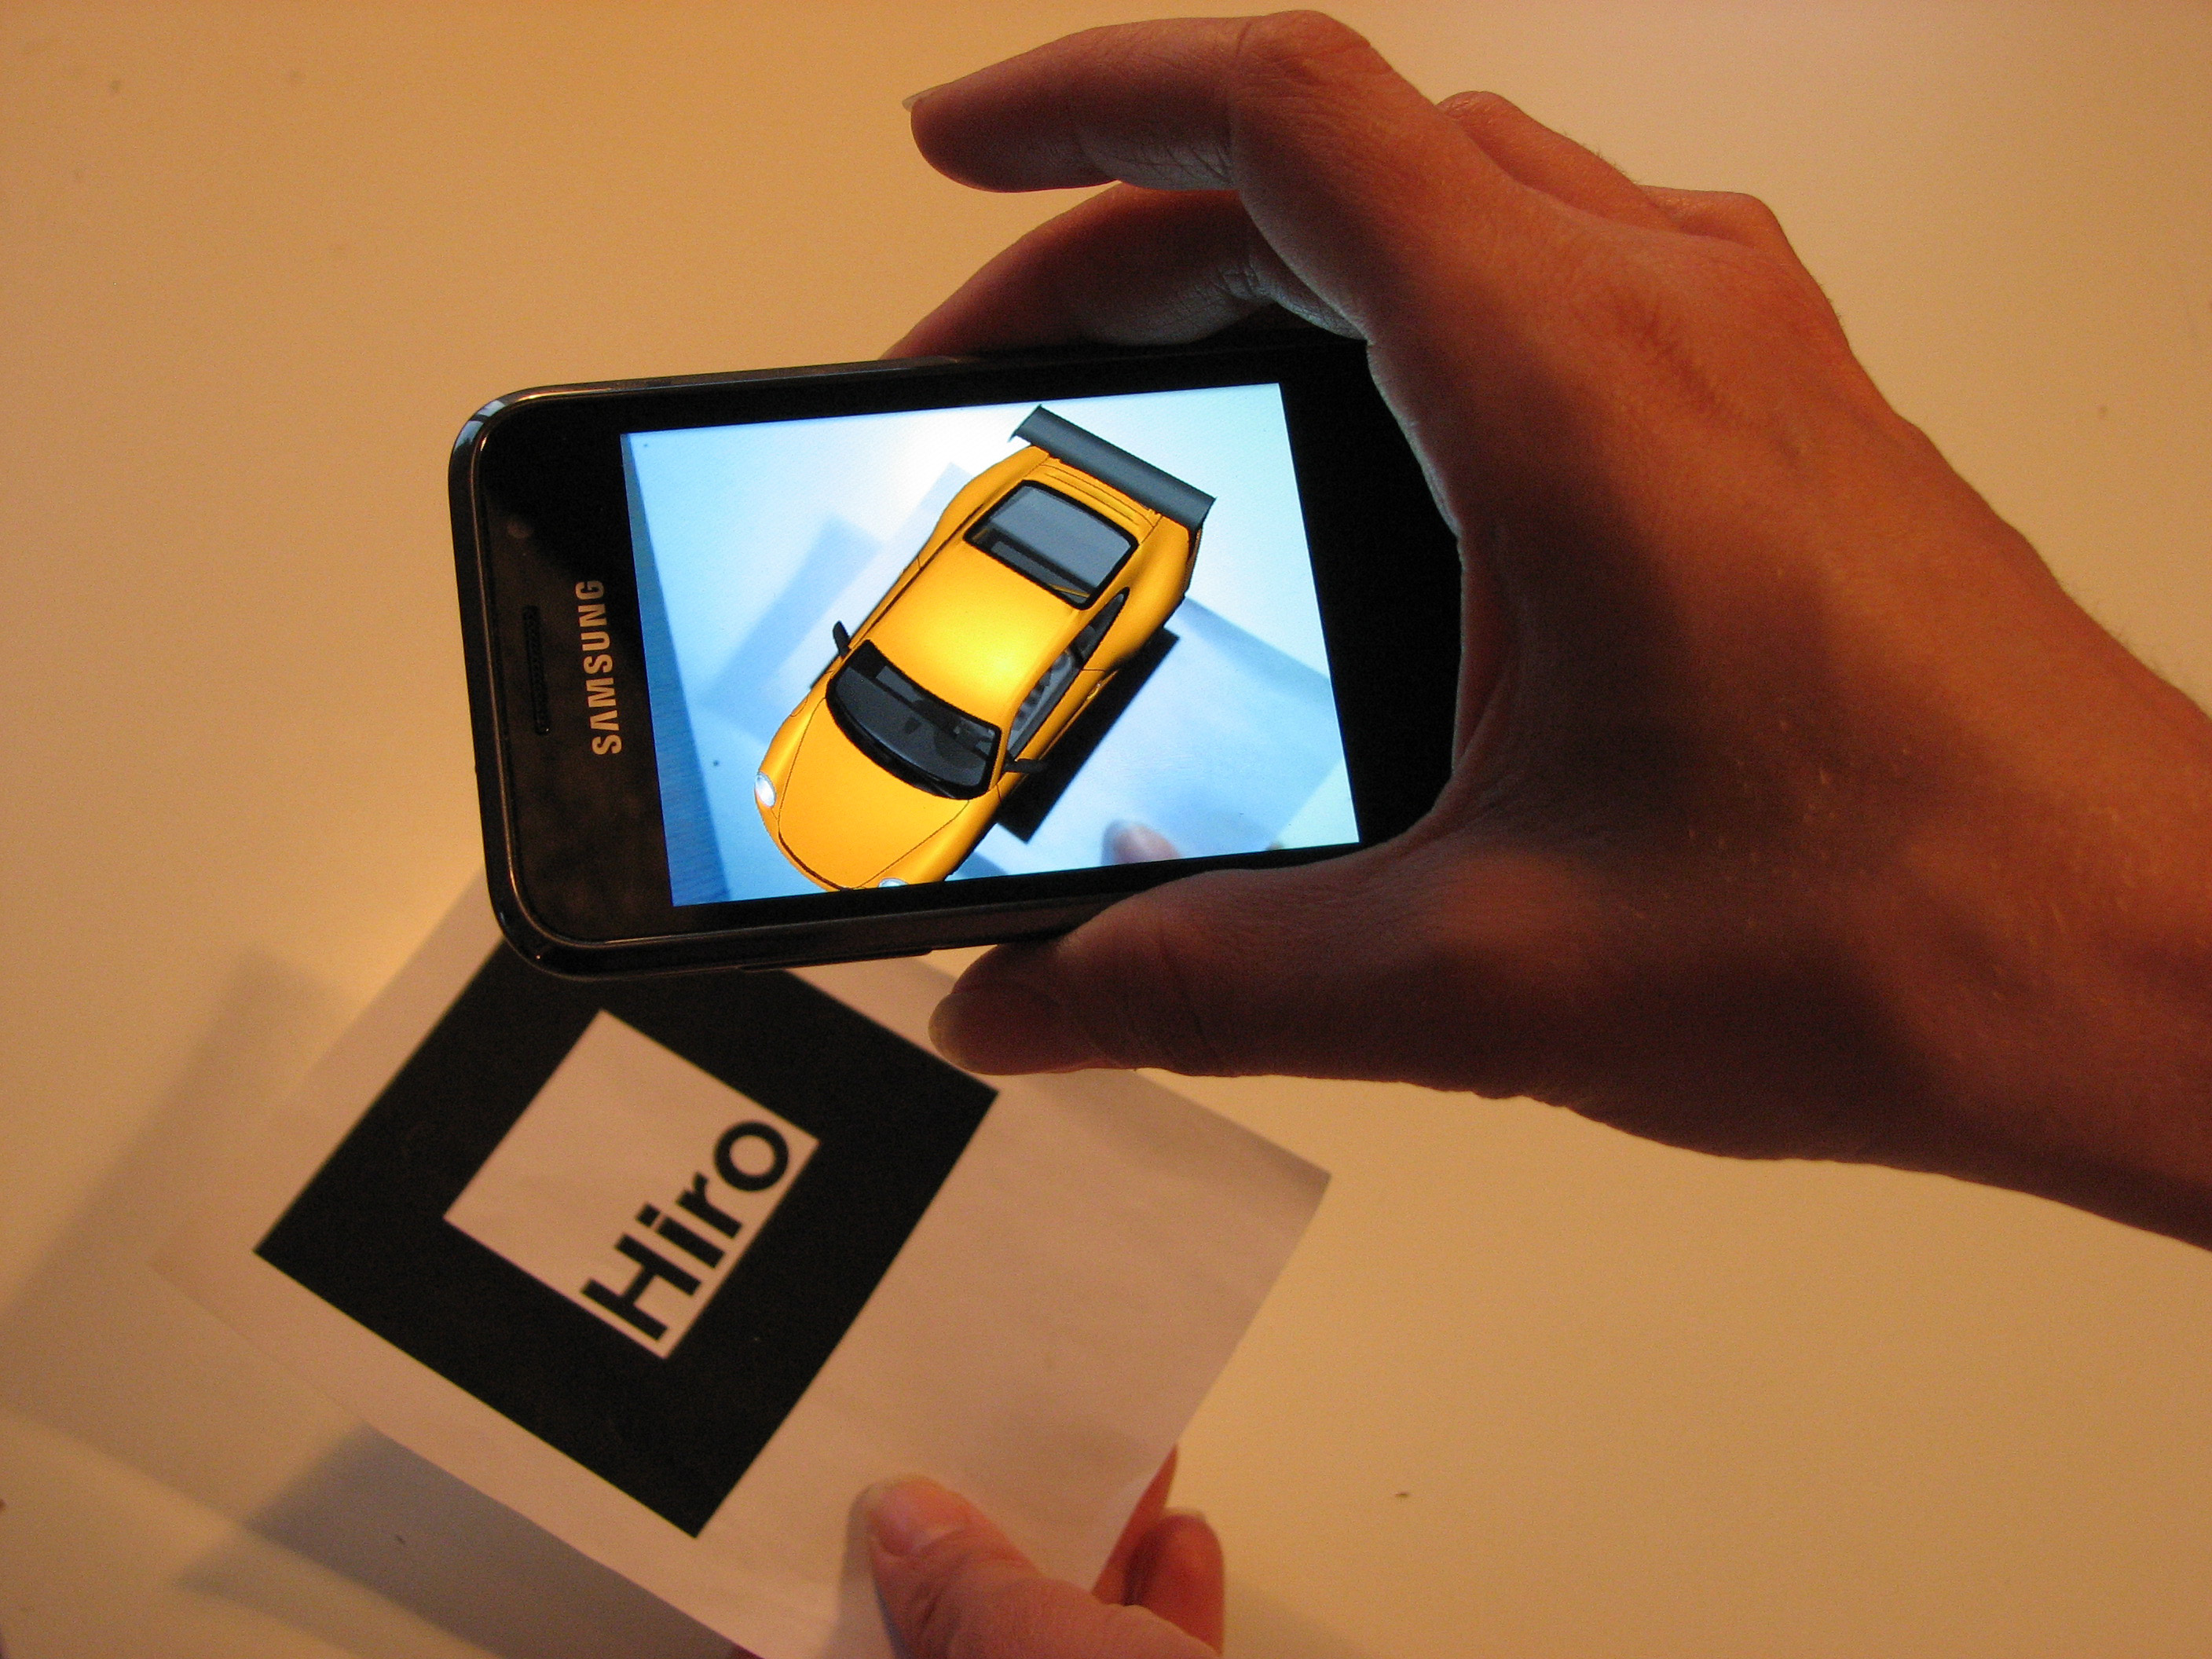
\includegraphics[scale=0.1]{figuras/cap2/ARToolKit-car-Android.jpg}
		\caption{\textit{Exemplo de utilização de smartphone na Realidade Aumentada~\cite{arToolWorks}.}}
		\label{fig:arAndroid}
	\end{figure}